\section{Empirical Results}\label{sec:exper}




The proofs in the previous sections were done with respect to the \textit{unit sphere}.  Although mathematically the results remain equally true for a sphere of radius $\mathcal{R}$, a natural question to raise is whether they remain \textit{practically} true in this setting.  If we view the idealized Earth as a sphere with  $\mathcal{R}=4000\text{ miles}$ and observe that the regions we are often interested in measuring are relatively small compared to the total surface area, then it could be the case that any map projection still distorts the scores of the regions, but not by enough to change their ordering.  Here, we demonstrate that this is not the case, and that in practice the Polsby-Popper, convex hull, and Reock scores of the real Congresional districts are reordered by the map projections used in practice.\footnote{The code to compute the various compactness scores is based on Lee Hachadoorian's \textit{compactr} project \cite{hachadoorian2018reock}.}

Rather than computing the scores on the sphere, we compare the scores a pair of familiar map projections.  Since for any pair of map projections, if the induced score ordering under them is different, then at least one of the two projections must have permuted the score ordering.  The projections we compare are the \textit{Mercator} projection and the \textit{Latitude-Longitude} projection.  The Mercator projection is a cylindrical projection constructed by placing the sphere in the middle of a cylinder and projecting each point on the sphere outward onto the surface of the cylinder along the line passing through the point and the center of the sphere (see Figure~\ref{fig:mercator}).

\begin{figure}
    \centering
    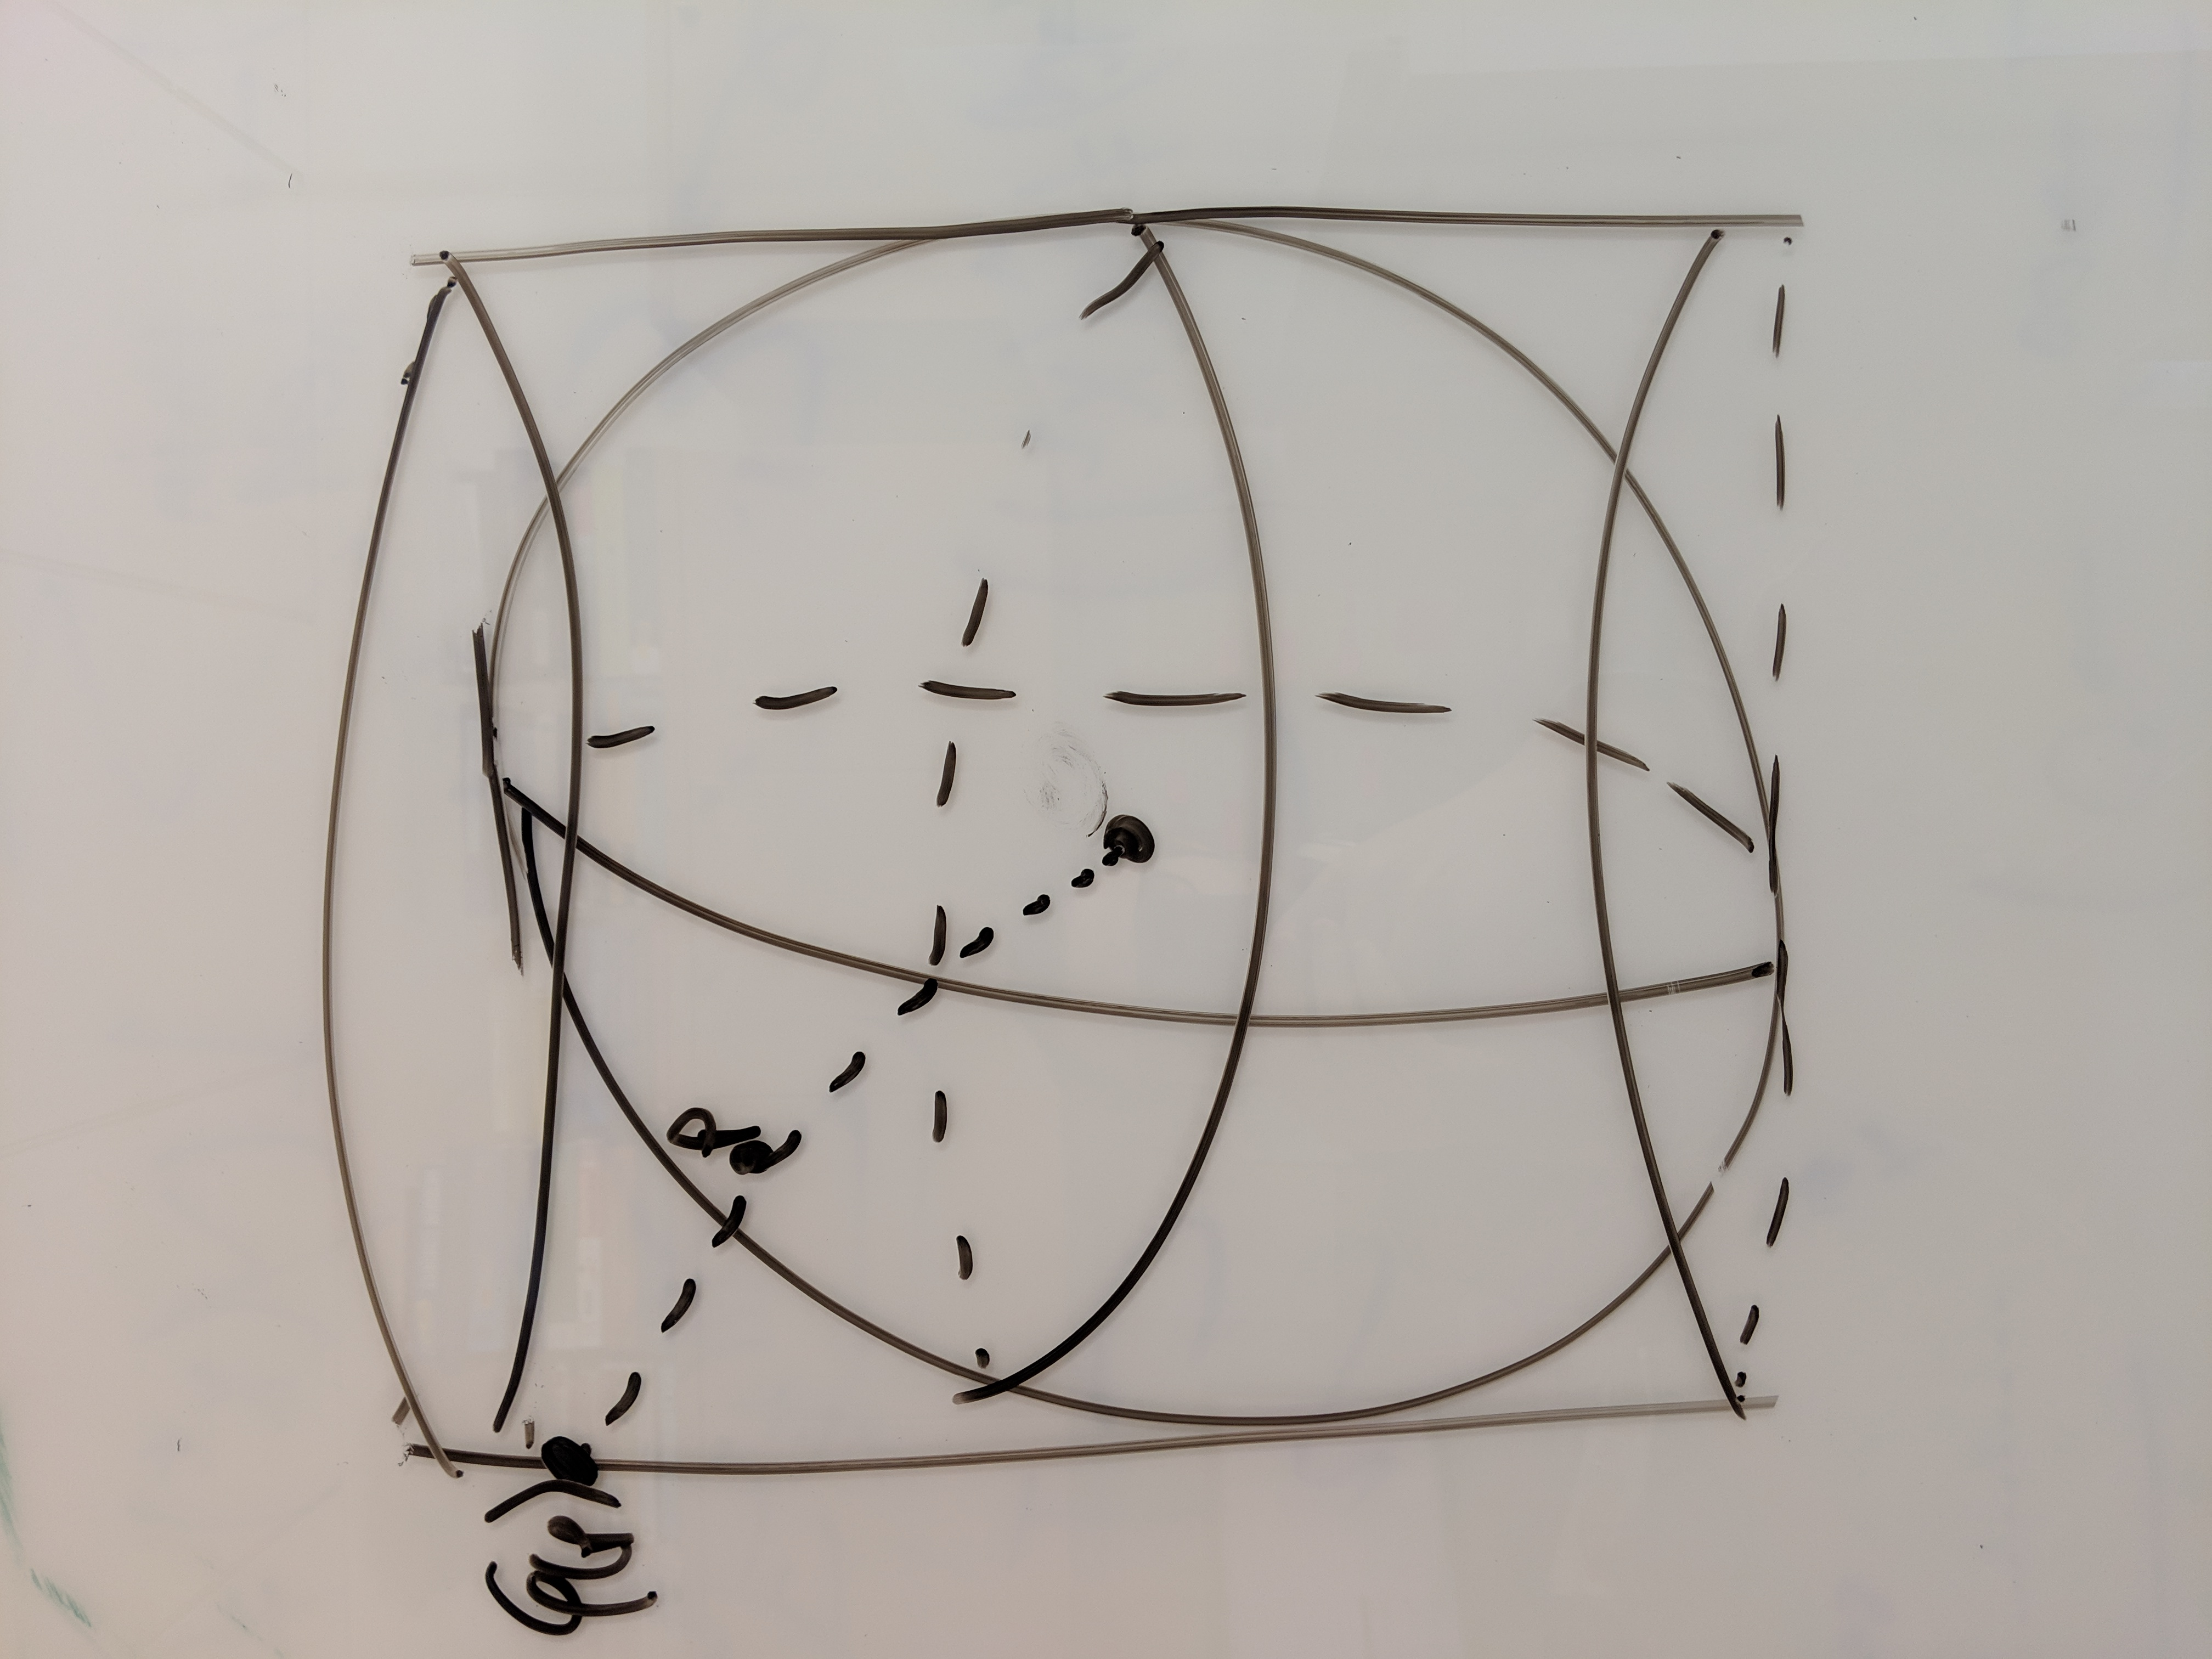
\includegraphics[width=.8\textwidth, angle=270,origin=c]{figs/merc.jpg}\\[1.5em]
    \caption{ A Mercator projection from the sphere to the surface of the cylinder.}
    \label{fig:mercator}
\end{figure}

This cylinder is then `unrolled' to a flat, planar map.  The Latitude-Longitude projection simply uses $(\mathit{\mathrm{lon}},\mathit{\mathrm{lat}})$ pairs as $(x,y)$ coordinates in the plane.  The Mercator and its variants, including the Universal Transverse Mercator and several state plane projections, is among the most commonly used projections.  The U.S. Census Bureau provides shapefiles for geographic entities in the United States, including Congressional districts, in a Latitude-Longitude coordinate reference system.\footnote{We use the U.S. Census Bureau's shapefile for the Congressional districts for the 115th Congress.  These are the districts in place for the 2016 election cycle.  Our Mercator projection is the WGS84 Spherical Mercator (EPSG:3857).  Our Latitude-Longitude projection is the NAD83 North American Latitude-Longitude (EPSG:4269).}


We first compare the three scores under the two projections for all\footnote{An astute reader will notice these plots have 434, points.  We omit the Alaska At-Large Congressional district since it crosses the International Date Line, which makes the convex hull and bounding circle hard to compute in a Latitude-Longitude projection.} districts in the country.  Each point represents one district.  The horizontal axis is the ordinal position with respect to the ordering induced by the score under the Latitude-Longitude projection and the vertical axis under the Mercator projection.  If both projections were to induce the same score ordering, every point would lie on the 45 degree line up the diagonal.


\begin{figure}[H]
\centering
\subfloat[Polsby-Popper]{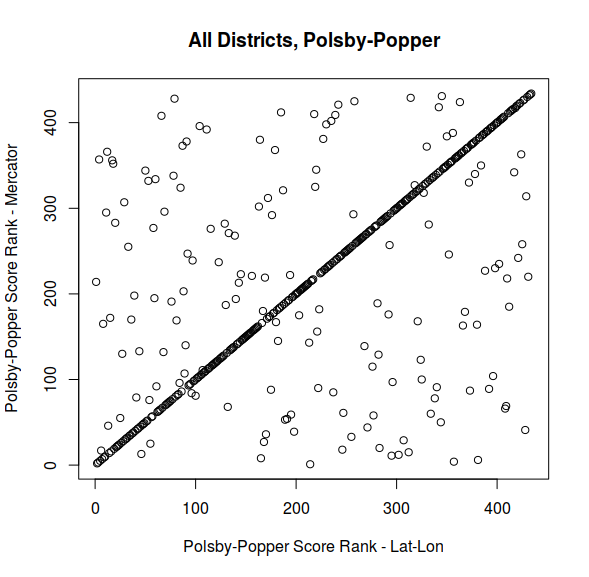
\includegraphics[width = .3\textwidth]{figs/all_pp.png}} 
\subfloat[Convex Hull]{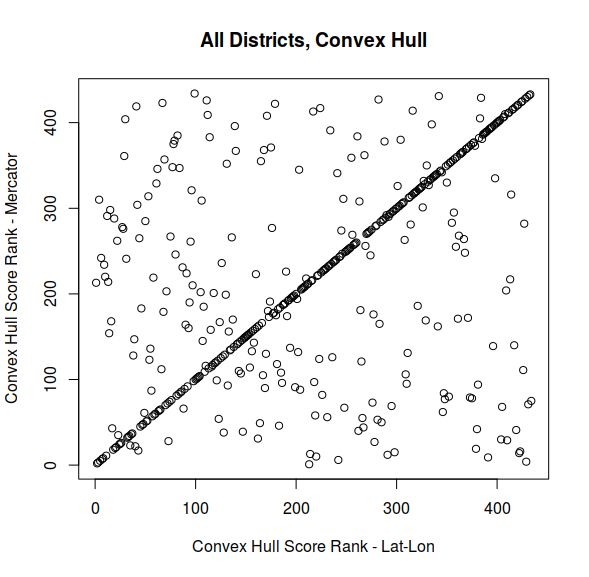
\includegraphics[width = .3\textwidth]{figs/all_ch.png}}
\subfloat[Reock]{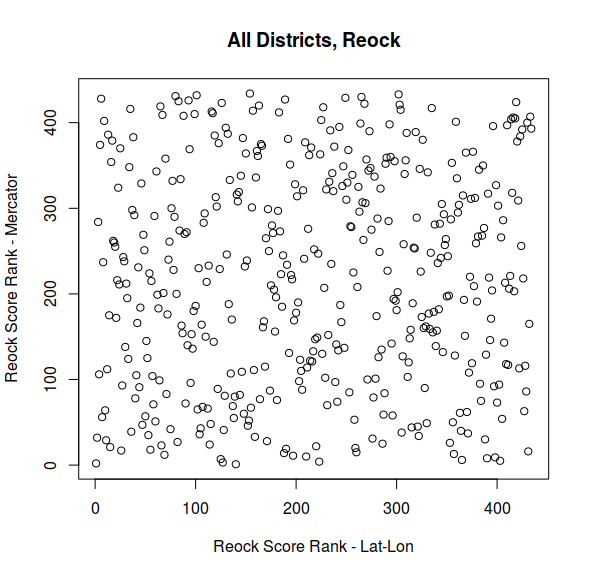
\includegraphics[width = .3\textwidth]{figs/all_reock.png}}\\[1.5em]

\caption{The permutation of compactness scores for all Congressional districts.}
\label{fig:allscores}
\end{figure}



While it is an illuminating exercise to demonstrate this effect across all districts, districting plans are proposed and evaluated on a state-by-state basis.  In the following plots, we restrict our attention to Texas, and observe a similar phenomenon.


\begin{figure}[H]
\centering
\subfloat[Polsby-Popper]{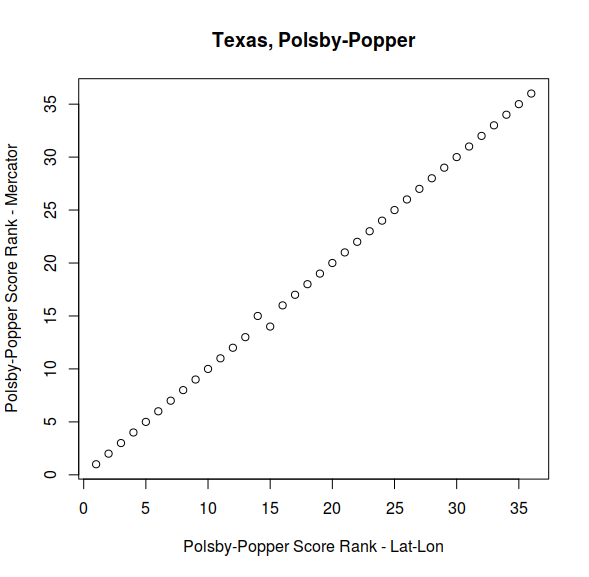
\includegraphics[width = .3\textwidth]{figs/texas_pp.png}} 
\subfloat[Convex Hull]{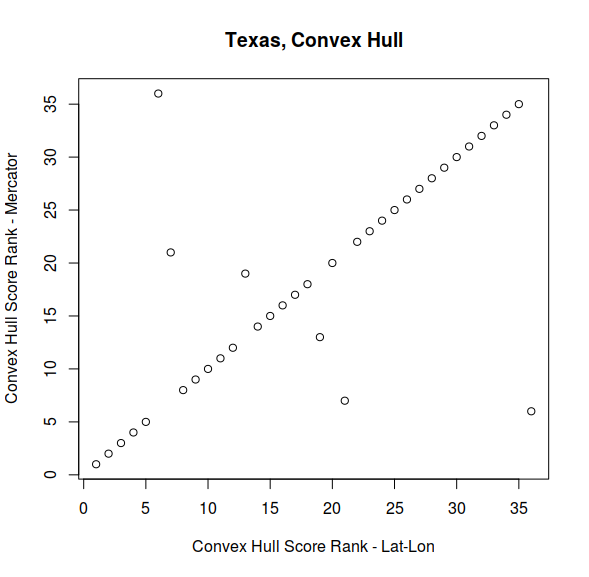
\includegraphics[width = .3\textwidth]{figs/texas_ch.png}}
\subfloat[Reock]{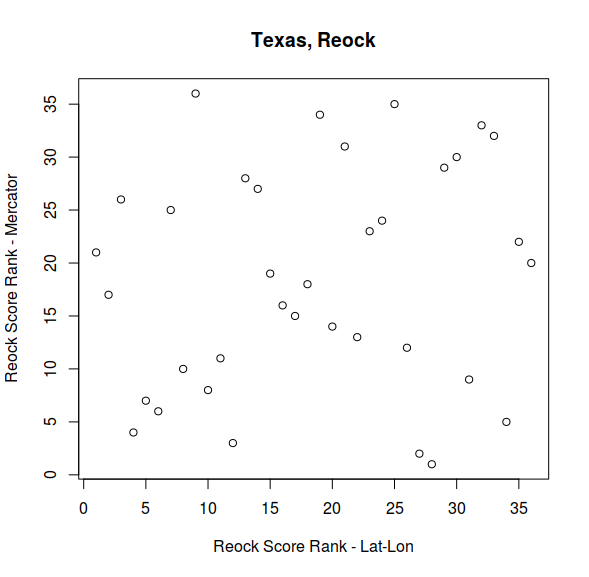
\includegraphics[width = .3\textwidth]{figs/texas_reock.png}}\\[1.5em]

\caption{The permutation of compactness scores for Texas' Congressional districts.}
\label{fig:txscores}
\end{figure}




We observe overall that the orderings of under the Polsby-Popper score and convex hull score are relatively undisturbed compared to that of the Reock score.  This is because the \textit{values} of those scores do not change by too much under different projections.  Intuitively, this is because while both projections distort shapes, they do so in a way that does not affect either of these scores by too much, since in the case of the Polsby-Popper score, the perimeter and area of the regions are changed in similar ways, and in the case of the convex hull score, the area of the convex hull of a region is distorted in the same way as the region itself, so the ratio of the areas is similar across projections.

However, the Reock score specifically requires constructing a minimum bounding circle, and this circle can be dramatically different under different map projections.  The Mercator projection sends caps on the sphere which aren't too close to the poles to regions in the plane which are very nearly circular, while the Latitude-Longitude projection visibly stretches all but the smallest circles on the equator.  For regions away from the equator, such as U.S. Congressional districts, this difference is significant enough to permute the ordering of Reock scores.


\zs{would be cool if we could make a Jupyter notebook or something available with this}